% What happens when a jitted function is called: the hit path stays in C++,
% only a miss goes back into R.
\documentclass[tikz, border=10pt]{standalone}
\usetikzlibrary{arrows.meta, positioning}

\begin{document}
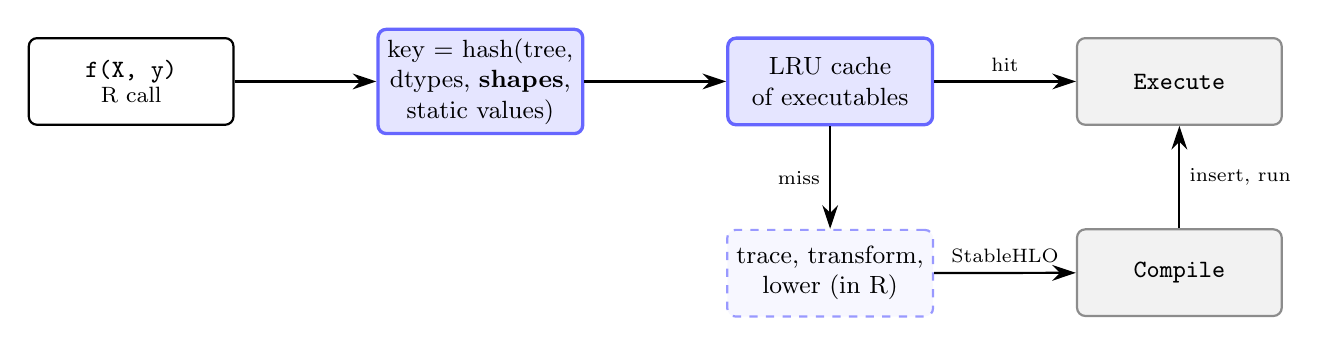
\begin{tikzpicture}[
  node distance=1.8cm,
  box/.style={
    draw, rounded corners=3pt, thick,
    minimum width=2.6cm, minimum height=1.1cm,
    align=center, font=\small
  },
  cpp/.style={box, fill=blue!10, draw=blue!60, very thick},
  rside/.style={box, fill=blue!3, draw=blue!40, dashed, thick},
  ext/.style={box, fill=black!5, draw=black!45},
  arr/.style={-{Stealth[length=3mm, width=2mm]}, thick},
  lab/.style={font=\scriptsize}
]
  \node[box] (call) {\texttt{f(X, y)}\\[-2pt]{\footnotesize R call}};
  \node[cpp, right=of call] (key)
    {key = hash(tree,\\dtypes, \textbf{shapes},\\static values)};
  \node[cpp, right=of key] (lru) {LRU cache\\of executables};
  \node[ext, right=of lru] (exec) {\texttt{Execute}};

  \node[rside, below=1.3cm of lru] (trace) {trace, transform,\\lower (in R)};
  \node[ext, below=1.3cm of exec] (compile) {\texttt{Compile}};

  \draw[arr] (call) -- (key);
  \draw[arr] (key) -- (lru);
  \draw[arr] (lru) -- node[above, lab] {hit} (exec);
  \draw[arr] (lru) -- node[left, lab] {miss} (trace);
  \draw[arr] (trace) -- node[above, lab] {StableHLO} (compile);
  \draw[arr] (compile) -- node[right, lab] {insert, run} (exec);
\end{tikzpicture}
\end{document}
